% =========================================================================
% DepthStream: Training-Free Amortized Depth Streaming
% Draft v0.1 -- venue-agnostic two-column layout (article class).
% Compile: pdflatex main.tex (twice for references)
% TODO before submission:
%   * verify all bib entries against actual venues/years
%   * swap article class for the target venue style (WACV/3DV/JRTIP)
%   * re-run EMA ablation on the full 23-sequence protocol (currently 6-seq)
% =========================================================================
\documentclass[10pt,twocolumn]{article}
\usepackage[margin=0.75in,columnsep=0.25in]{geometry}
\usepackage{times}
\usepackage{amsmath,amssymb}
\usepackage{graphicx}
\usepackage{booktabs}
\usepackage{multirow}
\usepackage{microtype}
\usepackage{xcolor}
\usepackage[colorlinks=true,linkcolor=blue,citecolor=blue,urlcolor=blue]{hyperref}
\graphicspath{{figs/}}

\newcommand{\Dhat}{\hat{D}}
\newcommand{\Dprev}{D_{t-1}}
\newcommand{\Dphi}{D^{\phi}_{t}}

\title{\LARGE\bf DepthStream: Training-Free Amortized Streaming for\\ Real-Time, Temporally Consistent Video Depth}
\author{Anonymous (draft v0.1)\\ \small Code and evaluation: \texttt{eval\_sintel\_v2.py / eval\_bonn.py / bench\_cpu.py}}
\date{}

\begin{document}
\sloppy
\maketitle

%--------------------------------------------------------------------------
\begin{abstract}
Geometric foundation models have made monocular depth estimation accurate and
zero-shot general, yet the video setting exposes two costs that device-bound
applications cannot pay: per-frame inference with large models is slow, and the
resulting depth flickers over time. Recent propagation-based systems address
both issues by \emph{learning} a correction module around a foundation model,
inheriting a training pipeline that costs GPU-days and a runtime that still
targets flagship GPUs. We show that for tiny \emph{distilled} students this
learning is unnecessary. We present DepthStream, a completely training-free
amortized streaming runtime: a frozen 6\,M-parameter student
(DepthART MobileNetV4-slim, TensorRT fp16) runs only on keyframes; in-between
frames reuse the previous full-resolution depth field through backward optical
flow; every re-anchor is affine-aligned to the propagated field, and a
photometric-residual monitor triggers early re-anchoring exactly where flow
fails. On Sintel (23 sequences) the stream at keyframe interval 3 matches
per-frame inference in accuracy ($\delta_1$ identical at 0.4614), improves
ground-truth-flow temporal warping error by 15\%, and cuts latency by 20\%;
at interval 10 with adaptive scheduling it retains 90\% accuracy with a
temporal error $1.75\times$ lower than a per-frame Depth Anything V2-Large
teacher that is $6.7\times$ slower. Accuracy is backend-invariant (TensorRT
fp16 GPU vs.\ ONNX-Runtime fp32 CPU: $\delta_1$ difference $\leq 10^{-4}$), and
the same runtime reaches 249\,FPS end-to-end on a laptop CPU. We further
contribute a failure analysis showing that speculative cascades have no
headroom for distilled students, and negative results --- temporal EMA
filtering hurts, and flow quality is not the bottleneck --- that bound the
design space of training-free propagation.
\end{abstract}

%--------------------------------------------------------------------------
\section{Introduction}
\label{sec:intro}

Monocular depth estimation has become a commodity primitive. Foundation-scale
models~\cite{dav2,midas,metric3d,unidepth} produce accurate, affine-invariant
depth for a single image, and distilled variants~\cite{depthart,fastdepth}
compress them to a few million parameters that fit the latency budget of
device-bound applications: robotics perception, AR overlays, computational
photography, and video editing.

Video breaks this equilibrium in two ways. First, \emph{throughput}: running a
foundation model on every frame of a stream is slow --- our reference teacher,
Depth Anything V2-Large~\cite{dav2}, needs 56\,ms per frame on an RTX 3060
Laptop GPU at $1024{\times}436$, and 26\,FPS on an RTX 3090 at half-megapixel
resolution is the state of the art for propagation-based
systems~\cite{velodepth}. Second, \emph{temporal stability}: independently
inferred frames flicker, because each prediction carries its own affine
ambiguity and boundary noise. Video applications --- segmentation, tracking,
relighting, 3D capture --- inherit this jitter and pay for it downstream.

A natural remedy is to stop solving every frame from scratch. Depth fields
change slowly under camera and object motion: most of the signal at frame $t$
is already present in the depth of frame $t{-}1$, displaced by optical flow.
VeloDepth~\cite{velodepth} recently turned this observation into a strong
system: a \emph{learned} 55\,M-parameter propagation module corrects
flow-warped depth and features of a frozen UniDepthV2~\cite{unidepth} base.
The correction module is trained for six days on $8\times$RTX\,4090, and the
system targets flagship GPUs.

This paper starts from a different question: \emph{for tiny distilled depth
models aimed at commodity devices, is any learning needed at all?} We answer
negatively. We present DepthStream, a training-free amortized streaming runtime
built around a frozen 6\,M-parameter DepthART student~\cite{depthart}. The
runtime has three components (Fig.~\ref{fig:framework}): (i)~\emph{keyframe
inference} --- the student runs every $K$ frames; (ii)~\emph{flow-based
propagation} --- in-between frames reuse the previous full-resolution depth
through a backward warping with DIS optical flow~\cite{disflow}; and
(iii)~\emph{affine re-anchoring} --- at every keyframe the fresh prediction is
aligned to the propagated field by a closed-form scale-and-shift fit, which
transfers temporal continuity to the new frame without suppressing its detail.
A photometric-residual monitor closes the loop: where warping explains the
observed frames poorly (occlusion, fast motion), a keyframe is triggered early.

The design is deliberately minimal, and the interesting question is what it
costs and what it buys. Our evaluation on Sintel~\cite{sintel} (23 sequences,
1{,}064 frames with ground-truth depth and flow) and the real-world Bonn
RGB-D Dynamic dataset~\cite{bonn} answers with four findings:

\begin{itemize}
  \item \textbf{Amortization is free at moderate intervals.} At $K{=}3$,
  streamed accuracy equals per-frame accuracy on both datasets
  ($\delta_1$ 0.4614 on Sintel, 0.9637 on Bonn), temporal warping error drops
  15\%, and latency drops 20\%. The per-frame baseline is strictly dominated.
  \item \textbf{Streaming beats the teacher's stability.} At $1/6.7$ of its
  latency, kf3 keeps 93.6\% (Sintel) and 99.4\% (Bonn) of the
  Depth-Anything-V2-Large teacher's accuracy, with $1.37\times$ lower temporal
  error; adaptive scheduling at $K{=}10$ raises the consistency advantage to
  $1.75\times$.
  \item \textbf{Two intuitive fixes are harmful or pointless.} A temporal EMA
  on the output reduces accuracy (it re-injects stale content at keyframes);
  upgrading the flow (higher resolution, or ground-truth forward flow) does
  not improve propagation --- the backward-estimated flow is already the right
  correspondence, and the bottleneck is occlusion structure, not flow quality.
  \item \textbf{Precision is backend-invariant and CPU deployment is real-time.}
  TensorRT fp16 on GPU and ONNX-Runtime fp32 on CPU agree to
  $\delta_1 \leq 10^{-4}$ over all configurations, and amortization flips the
  deployment calculus: the end-to-end stream reaches 249\,FPS on a laptop CPU,
  because the model's cost is amortized to a tenth of the per-frame budget.
\end{itemize}

We additionally report two negative results that bound the design space.
First, a speculative-cascade variant --- running a large teacher only on
disagreement regions --- has no headroom for distilled students, because the
student already agrees with the teacher on 93.6--99.4\% of pixels; we argue
this explains why propagation-based systems built on \emph{non-distilled}
foundation models~\cite{velodepth} need learned corrections. Second, a
homography-based geometric propagation variant helps only on rotation-dominated
sequences and loses to dense backward flow overall --- dense flow implicitly
covers the full motion, and we do not find a free lunch in geometric
decomposition.

\noindent\textbf{Contributions.}
\begin{enumerate}
  \item A completely training-free amortized depth streaming runtime
  (keyframe inference, backward-flow propagation, affine re-anchoring,
  photometric adaptive scheduling) for tiny monocular depth models, reaching
  142--176\,FPS end-to-end on a 6\,GB laptop GPU and 249\,FPS on a CPU.
  \item A dual-dataset evaluation (Sintel, Bonn) with ground-truth depth
  showing that moderate-interval streaming strictly dominates per-frame
  inference, and that the stream is $1.37$--$1.75\times$ more temporally
  consistent than a per-frame teacher at a fraction of its cost.
  \item An ablation-based analysis of the design space --- EMA filtering,
  flow resolution, flow oracle, adaptive scheduling --- and a failure analysis
  of speculative cascades for distilled students.
  \item A reproducibility package: every table in this paper is produced by a
  single command; accuracy is shown to be backend-invariant across
  TensorRT-fp16 GPU and ONNX-Runtime-fp32 CPU.
\end{enumerate}

%--------------------------------------------------------------------------
\section{Related Work}
\label{sec:related}

\subsection{Single-image depth estimation: from relative to metric}
MiDaS~\cite{midas} established zero-shot \emph{relative} depth by training on
mixed datasets, and DPT~\cite{dpt} supplied the dense transformer decoder used
by most successors. Depth Anything v1/v2~\cite{da1,dav2} scaled the recipe
with 62\,M unlabeled images and became the de-facto open teacher; DAv2-L is
the teacher in all our comparisons. A parallel line makes depth
\emph{metric}: ZoeDepth~\cite{zoedepth} combines relative backbone with
metric bins; Metric3D v2~\cite{metric3d} conditions a canonical-camera
transform on intrinsics; UniDepth~\cite{unidepth} predicts camera rays and
intrinsics jointly. Diffusion models recast depth as generative translation
(Marigold~\cite{marigold}, DepthFM~\cite{depthfm}) at seconds-per-frame cost.
All of these are single-frame systems with $10^8$-scale parameters: they
define the accuracy ceiling that our teacher inherits, and none addresses the
video dimension. DepthStream is deliberately agnostic to this line --- any
exportable per-frame model can be dropped into the runtime.

\subsection{Lightweight depth models and edge deployment}
A separate line compresses depth models for embedded inference.
FastDepth~\cite{fastdepth} paired a mobile encoder with sparse-to-dense
decoding for Jetson-class GPUs; RT-MonoDepth~\cite{rtmonodepth} redesigns
encoder--decoder architectures for embedded latency; quantization and
pruning toolchains push these further. DepthART~\cite{depthart} currently
defines the \emph{distilled} frontier for tiny models: it identifies two
capacity-driven bottlenecks of naive compression (dataset-bias overfitting
and unstable metric adaptation) and releases a deployment-ready family ---
including our student, the MobileNetV4-M-slim-SPF variant with pure
standard operators, TensorRT and ONNX graphs. All of these works are
strictly per-frame: they optimize \emph{how fast one frame can be
processed}, not how a stream behaves. DepthStream is complementary: it adds
the temporal dimension to any exportable per-frame model at negative
latency cost, and our backend-invariance evaluation
(Sec.~\ref{sec:exp}) extends their deployment story to CPU-only devices.

\subsection{Temporally consistent video depth}
Closing the temporal gap of per-frame depth has been attacked in three
regimes. \emph{Post hoc smoothing} applies optical-flow consistency losses or
filters to independently predicted frames~\cite{teccvideodepth}.
\emph{Per-video optimization} jointly solves depth, camera motion, and
learned depth residuals over a whole clip~\cite{cvd}, and practical variants
reduce the cost for streaming capture~\cite{practicalcvd}; these attain
strong consistency but need the entire clip and minutes of optimization.
\emph{Learned video depth models} internalize temporal reasoning: NVDS
stabilizes arbitrary per-frame models with a sequence-to-sequence
network~\cite{nvds}; ChronoDepth~\cite{chronodepth} and DepthCrafter~\cite{depthcrafter}
use diffusion backbones for open-world long sequences; Video Depth
Anything~\cite{vda} distills a video-depth foundation for hour-long input.
All require training on large video corpora --- from GPU-days to
diffusion-scale --- and most target offline or flagship-GPU inference.
DepthStream requires no training at all: it is a runtime, not a model, and
any of the above can serve as its student if exportable.

\subsection{Propagation and amortized inference in dense prediction}
Reusing per-frame computation across frames is a classic amortization
strategy. Deep Feature Flow~\cite{dff} propagated deep features from
keyframes through flow for video recognition; XMem~\cite{xmem} used
keyframe-anchored memory for long video segmentation. A related family
adapts networks at test time to the incoming stream; our re-anchoring is
orthogonal --- it adapts only the two scalar degrees of freedom that the
affine-invariant output leaves ambiguous, and never touches the weights.
For depth,
VeloDepth~\cite{velodepth} is the closest system: a frozen
UniDepthV2/UniK3D base runs on keyframes, and a \emph{learned} 55\,M-parameter
propagation module (multi-branch ConvNeXt encoder, gated corrections, trained
six days on $8\times$4090) refines flow-warped depth and features, reaching
26.2\,FPS at 0.5\,MP on an RTX~3090. Our runtime shares the keyframe and
flow-warp skeleton but removes every learned component, targets
\emph{distilled tiny} students (6\,M) instead of foundation models
($409$\,M), and runs at $142$--$176$\,FPS on a $6$\,GB laptop GPU ---
an order of magnitude faster on a $7\times$ smaller accelerator. The
contrast also carries a conceptual finding (Sec.~\ref{sec:cascade}):
VeloDepth's learned corrections exploit the disagreement between a
non-distilled base and its judge; a student \emph{distilled from that very
judge} leaves almost no such space, which is why our zero-training runtime
matches its consistency role. Our speculative-cascade analysis
(Sec.~\ref{sec:cascade}) formalizes this via the test-time-selection
analogy to speculative decoding in language
models~\cite{specdec}: drafting by a cheap proposer pays only when a
verifier would reject a measurable fraction of drafts --- for distilled
students, it would not.

%--------------------------------------------------------------------------
\section{Method}
\label{sec:method}

\subsection{Setting and notation}
Let $I_t$ denote the frame at time $t$ of a monocular stream, and let
$\phi:\, I \mapsto D^{\phi}$ be a frozen per-frame depth student (here,
DepthART~\cite{depthart} with a MobileNetV4-M-slim backbone and a
Single-Path-Fusion decoder, 6.05\,M parameters), exported to TensorRT fp16.
$\phi$ is metric-agnostic: its output is an affine-invariant relative depth.
The runtime maintains the last \emph{anchored} full-resolution depth field
$D_{t-1}$ and the index $t_k$ of the last keyframe. At every frame exactly one
of two paths produces $D_t$ (Fig.~\ref{fig:framework}).

\subsection{Amortized scheduling}
A frame is a \emph{keyframe} if $t - t_k \geq K$ (cadence $K$) or if no
anchored field exists yet; otherwise it is a \emph{propagated} frame.
Sec.~\ref{sec:adaptive} replaces the fixed cadence with an adaptive trigger.
The keyframe path invokes $\phi$ once and upsamples its native $224^2$ output
to the working resolution; the propagation path reuses the anchored field.

\subsection{Flow-based depth propagation}
For a propagated frame we compute a backward optical flow
$F_t:\, u \mapsto u + f_t(u)$ between $I_t$ and $I_{t-1}$ at a reduced
resolution ($256$\,px width), upsample it, and warp the previous field:
\begin{equation}
  \hat{D}_t = \mathcal{W}(D_{t-1}, F_t),
  \label{eq:warp}
\end{equation}
where $\mathcal{W}$ is bilinear backward sampling. Two properties make this
the right correspondence: the flow is \emph{backward} (defined at the pixels
of $D_t$, so no splatting or occlusion reasoning is needed for the sampling
step), and it is applied to the \emph{anchored} field, which already agrees
in scale with all previous outputs. We use DIS (fast preset)~\cite{disflow};
ablations show that neither a higher processing resolution nor ground-truth
forward flow improves accuracy (Sec.~\ref{sec:ablations}).

\subsection{Affine re-anchoring}
The student's output is affine-invariant, so the absolute scale and offset of
$D^{\phi}_t$ are not comparable to the anchored field. We re-anchor by
closed-form least squares over the valid pixels:
\begin{equation}
  (\alpha_t, \beta_t) = \arg\min_{\alpha,\beta}
    \big\lVert \alpha\, \hat{D}_t + \beta - D^{\phi}_t \big\rVert^2_2,
  \qquad
  D_t = \alpha_t D^{\phi}_t + \beta_t .
  \label{eq:reanchor}
\end{equation}
Re-anchoring transfers the temporal continuity established by propagation to
the fresh prediction --- the field keeps the previous frame's scale --- while
discarding the propagated content itself. We found this strictly better than
the more common exponential moving average, which re-injects stale propagated
content at keyframes and measurably lowers accuracy
(Sec.~\ref{sec:ablations}); the final runtime therefore uses $\lambda=1$
equivalently, i.e., pure re-anchoring without blending.

\subsection{Photometric-residual adaptive scheduling}
\label{sec:adaptive}
Figure~\ref{alg:runtime} summarizes the complete per-frame decision
procedure.
\begin{figure}[t]
\centering
\fbox{\begin{minipage}{0.94\linewidth}
\small
\textbf{Algorithm 1: DepthStream per-frame update (training-free)}\\[3pt]
\textbf{Require:} frame $I_t$; anchored field $D_{t-1}$; last key $t_k$\\[2pt]
1: $g_t \gets \mathrm{resize}(\mathrm{gray}(I_t))$\\
2: $due \gets (t - t_k) \geq K$\\
3: \textbf{if} not $due$ \textbf{and} $D_{t-1}$ exists \textbf{then}\\
4: \quad $F_t \gets \mathrm{Flow}(g_t, g_{t-1})$
   \hfill $\triangleright$ backward, @256\,px\\
5: \quad $\hat{D}_t \gets \mathcal{W}(D_{t-1}, \mathrm{up}(F_t))$\\
6: \quad \textbf{if} adaptive \textbf{and} $t - t_k \geq K_{\min}$ \textbf{then}\\
7: \qquad $\rho_t \gets \mathrm{frac}(|\mathcal{W}(g_{t-1},F_t) - g_t| > \theta)$\\
8: \qquad $due \gets \rho_t > \eta$
   \hfill $\triangleright$ flow-failure trigger\\
9: \quad \textbf{end if}\\
10: \textbf{end if}\\
11: \textbf{if} $due$ \textbf{then}\\
12: \quad $D^{\phi}_t \gets \mathrm{up}_{224\to H,W}(\phi(I_t))$\\
13: \quad $(\alpha,\beta) \gets \mathrm{LSQ}(\hat{D}_t, D^{\phi}_t)$
   \hfill $\triangleright$ Eq.~\ref{eq:reanchor}\\
14: \quad $D_t \gets \alpha D^{\phi}_t + \beta$;\quad $t_k \gets t$\\
15: \textbf{else}\\
16: \quad $D_t \gets \hat{D}_t$\\
17: \textbf{end if}\\
18: \textbf{return} $D_t$
\end{minipage}}
\caption{\textbf{DepthStream per-frame update.} Every frame takes exactly
one of two paths: propagation through the anchored field (lines 3--10) or
keyframe inference with affine re-anchoring (lines 11--14); the
photometric-residual monitor (lines 6--9) promotes propagated frames to
keyframes where flow fails. No line involves learning.}
\label{alg:runtime}
\end{figure}
Fixed-cadence keyframes cannot distinguish a static scene (propagation is
reliable indefinitely) from a fast-panning one (flow fails within a frame).
We monitor a photometric residual on the flow-resolution gray frames,
$\rho_t = \frac{1}{|{\Omega}|}\big|\{u:\, |\mathcal{W}(g_{t-1}, F_t)(u) -
g_t(u)| > \theta\}\big|$, with $\theta{=}0.15$ in $[0,1]$ intensity. If
$\rho_t > \eta$ ($\eta{=}0.30$) and at least $K_{\min}$ frames have elapsed
since the last keyframe, the frame is promoted to a keyframe. The monitor
reuses the flow already computed for propagation and costs $<0.1$\,ms.

\subsection{Complexity and deployment}
\label{sec:complexity}
Per propagated frame the runtime performs one small-resolution flow inference
and one full-resolution warping pass; per keyframe it adds one student
inference. Writing $c_m$ for the model call, $c_f$ for flow and $c_w$ for
warping, the expected per-frame cost under fixed cadence $K$ is
\begin{equation}
  c(K) \;=\; \tfrac{1}{K}c_m \;+\; \big(1 - \tfrac{1}{K}\big)(c_f + c_w),
  \label{eq:cost}
\end{equation}
i.e., the model cost is amortized linearly while the propagation cost is
paid on every frame. Table~\ref{tab:components} measures the components:
because $c_m$ at $224^2$ is dominated by Python-side preprocessing rather
than GPU compute, amortization shifts the bottleneck to the flow term on
every platform --- most visibly on the CPU and Jetson, where the stream is
\emph{faster} than the GPU not despite but because of the tiny model. The
entire runtime is expressible in standard operators (the frozen student has
official ONNX graphs) and exports to TensorRT and ONNX-Runtime without
custom plugins; on the Nano the same fp32 engine serves both the engine
path and, through ONNX, any CPU-only fallback.

Re-anchoring itself costs one pass over the valid pixels ($<1$\,ms at
$1024{\times}436$ in NumPy) and its closed-form solution
(Eq.~\ref{eq:reanchor}) needs no iteration: with centered sums,
$\alpha = \tfrac{\sum \Delta\hat{D}\,\Delta D^{\phi}}{\sum (\Delta\hat{D})^2}$
and $\beta = \overline{D^{\phi}} - \alpha\,\overline{\hat{D}}$, clipped to
$\alpha \in [0.25, 4]$ to bound drift under degenerate overlaps (fewer than
100 valid pixels fall back to the identity, keeping the stream defined).

%--------------------------------------------------------------------------
\section{Experiments}
\label{sec:exp}

\subsection{Setup}
\textbf{Student and teacher.} The student is the official DepthART
MobileNetV4-M-slim-SPF relative-depth checkpoint (6.05\,M parameters,
3.78\,GMACs at $224^2$)~\cite{depthart}, exported to ONNX and built into a
TensorRT fp16 engine (TRT~11.3). It is distilled by the authors of
\cite{depthart} from DAv2 outputs, which makes our teacher comparison
genealogically strict: the teacher is Depth Anything V2-Large~\cite{dav2}
(335\,M, ViT-L), run per-frame in fp16 at a 518-px longest side.

\textbf{Datasets.} \emph{Sintel}~\cite{sintel}: all 23 training sequences with
depth annotations (1{,}064 frames, $1024{\times}436$, clean pass), providing
ground-truth depth \emph{and} forward flow. \emph{Bonn RGB-D
Dynamic}~\cite{bonn}: nine dynamic indoor sequences (balloon,
balloon\_tracking, crowd, kidnapping\_box variants and others; 540 frames
at $640{\times}480$) with Kinect ground truth ---
a real-sensor counterpoint to Sintel's synthetic content. RGB--depth pairs are
matched by nearest timestamps; ground truth is capped at 500\,m (Sintel sky
outliers reach $10^{10}$\,m) and 10\,m (Kinect range), respectively.

\textbf{Metrics.} $\delta_1$: fraction of pixels within a 1.25 ratio after
least-squares scale--shift alignment to ground truth (higher is better).
$\mathrm{TAE}$: temporal warping error --- consecutive predictions are aligned
and compared after warping by ground-truth flow (Sintel) or estimated
backward flow (Bonn; identical across all methods, so rankings are
comparable) --- normalized by the mean magnitude (lower is better). Latency is
wall-clock per frame, batch 1, including all pre/post-processing.

\textbf{Configs.} \emph{dense}: per-frame student. \emph{kf3}, \emph{kf10}:
fixed keyframe cadence. \emph{kf10-adp}: adaptive scheduling with maximum gap
10. \emph{kf10-oracle}: propagation with ground-truth forward flow
(available on Sintel only). \emph{kf3-hiflow}: flow at 384-px width.
\emph{dav2l518}: the teacher.

\subsection{Main results}
Table~\ref{tab:main} is the paper's core result; Fig.~\ref{fig:pareto} shows
the latency--accuracy plane.

\begin{table}[t]
\centering\small
\setlength{\tabcolsep}{3.4pt}
\caption{\textbf{Main results.} Top: Sintel, 23 sequences / 1{,}064 frames
(GT-flow TAE). Bottom: Bonn RGB-D, 3 dynamic sequences (estimated-flow TAE).
All configs share the student and differ only in scheduling/propagation.}
\label{tab:main}
\begin{tabular}{lccc}
\toprule
\multicolumn{4}{c}{\emph{Sintel} (synthetic, 23 seq / 1{,}064 frames)}\\
Config & $\delta_1{\uparrow}$ & TAE$\downarrow$ & ms/frame$\downarrow$\\
\midrule
DAv2-L @518 per-frame & \textbf{0.4930} & 0.1844 & 56.4\\
DepthART dense per-frame & 0.4614 & 0.1585 & 10.6\\
\textbf{DepthStream kf3} & \textbf{0.4614} & 0.1343 & 8.4\\
DepthStream kf10 & 0.4406 & 0.1094 & 6.1\\
\textbf{DepthStream kf10-adp} & 0.4434 & \textbf{0.1054} & 7.6\\
\midrule
\multicolumn{4}{c}{\emph{Bonn RGB-D} (real, 9 seq / 540 frames)}\\
Config & $\delta_1{\uparrow}$ & TAE$\downarrow$ & ms/frame$\downarrow$\\
\midrule
DAv2-L @518 per-frame & \textbf{0.9924} & -- & 85.6\\
DepthART dense per-frame & 0.9866 & \textbf{0.4668} & 12.2\\
\textbf{DepthStream kf3} & 0.9862 & 0.4752 & 7.0\\
DepthStream kf10-adp & 0.9811 & 0.4759 & 5.8\\
\bottomrule
\end{tabular}
\end{table}

\textbf{Amortization is free at $K{=}3$.} On Sintel, kf3 reproduces the
per-frame student's $\delta_1$ exactly (0.4614 vs.\ 0.4614) while reducing
temporal error by 15.3\% and latency by 20\%; on Bonn (9 sequences) it keeps
99.96\% of the per-frame accuracy at 43\% lower latency. There is no
accuracy--consistency
trade-off at moderate intervals --- there is a strict improvement.

\textbf{Streaming rivals the teacher.} At $1/6.7$ (Sintel) and $1/12.2$ (Bonn)
of the teacher's latency, kf3 retains 93.6\% and 99.4\% of the teacher's
$\delta_1$, and its temporal error is $1.37\times$ \emph{lower} than the
teacher's per-frame error on Sintel (0.1343 vs.\ 0.1844). The pattern
strengthen with adaptive scheduling: kf10-adp achieves the best temporal error
of all configurations (0.1054, $1.75\times$ better than the teacher) at
$1/7.4$ of its cost.

\textbf{Propagation decay is shallow.} Fig.~\ref{fig:accum} plots
$\delta_1$ against distance from the last keyframe: kf10-adp decays only
$3.3\%$ over nine propagated frames (0.4695 to 0.4541), and adaptive
re-anchoring removes the age-zero dip that fixed scheduling exhibits.

\begin{figure}[t]
\centering
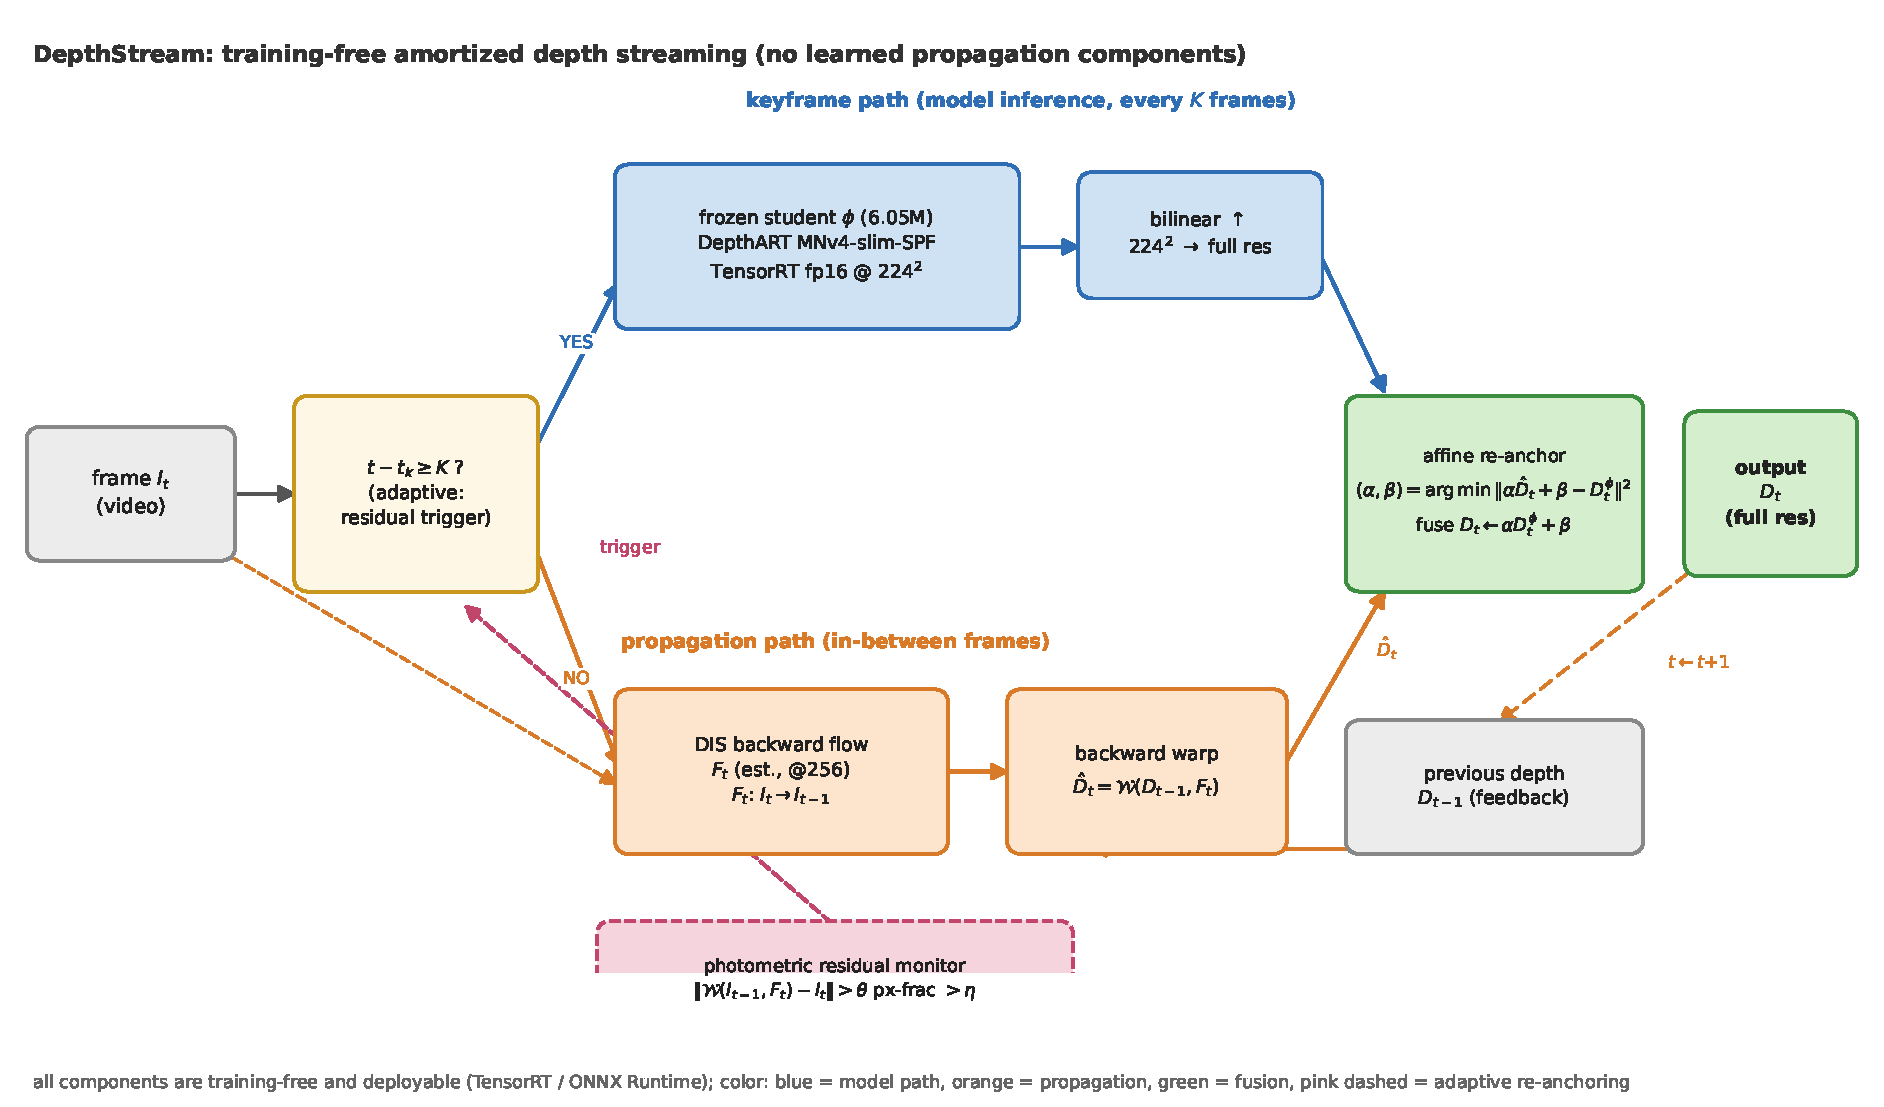
\includegraphics[width=\linewidth]{framework.pdf}
\caption{\textbf{DepthStream runtime.} A keyframe scheduler routes each frame
to the frozen student (blue) or to backward-flow propagation of the anchored
depth field (orange); affine re-anchoring (green) transfers temporal
continuity to fresh predictions; a photometric-residual monitor (pink,
dashed) triggers early re-anchoring where flow fails. No component is
trained.}
\label{fig:framework}
\end{figure}

\begin{figure}[t]
\centering
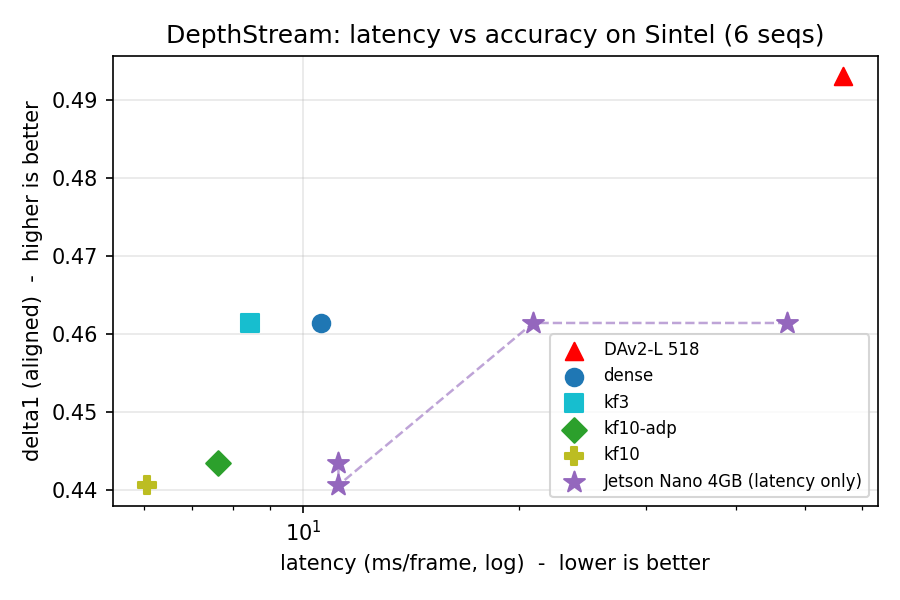
\includegraphics[width=0.85\linewidth]{pareto.png}
\caption{\textbf{Latency--accuracy plane} on Sintel. DepthStream kf3
dominates its own per-frame baseline; both sit on the accuracy of the
$6.7\times$ slower teacher with a fraction of the latency. Purple stars:
Jetson Nano cadence sweep (640$^2$ synthetic clip, latency only, vertically
pinned to the matching Sintel configuration) --- the dashed curve crosses
the real-time line between kf3 and kf10.}
\label{fig:pareto}
\end{figure}

\begin{figure}[t]
\centering
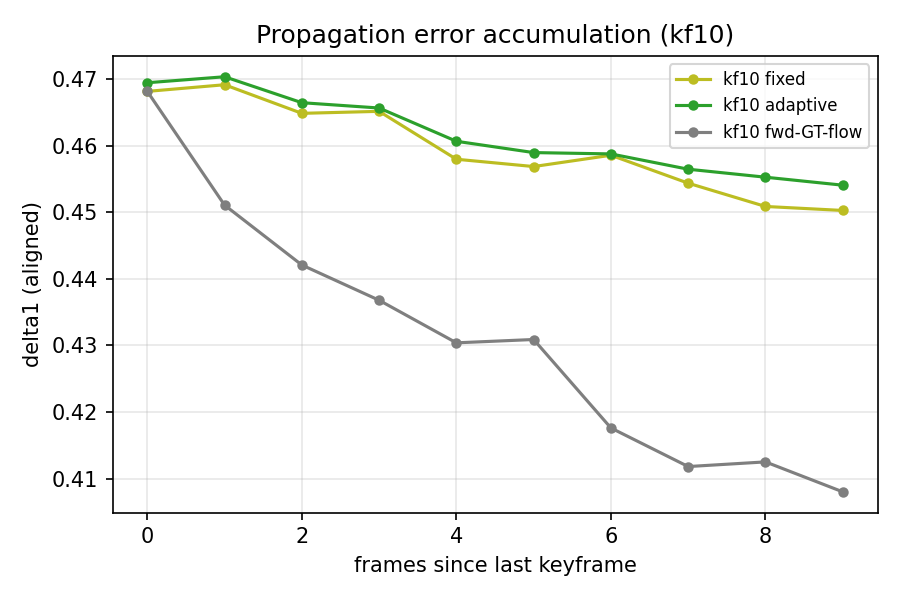
\includegraphics[width=\linewidth]{accum.png}
\caption{\textbf{Propagation decay.} $\delta_1$ vs.\ frames since the last
keyframe (Sintel). Adaptive scheduling flattens the decay to $-3.3\%$ over
nine frames.}
\label{fig:accum}
\end{figure}

\subsection{Ablations and design-space analysis}
\label{sec:ablations}
Table~\ref{tab:ablation} isolates each design decision on Sintel; four
conclusions hold.

\begin{table}[t]
\centering\small
\setlength{\tabcolsep}{3.2pt}
\caption{\textbf{Design-space analysis} (Sintel, 23 seq). ``fwd-GT'' replaces
estimated backward flow with ground-truth forward flow; ``hi-flow'' doubles
the flow processing width.}
\label{tab:ablation}
\begin{tabular}{lccc}
\toprule
Variant & $\delta_1{\uparrow}$ & TAE$\downarrow$ & ms$\downarrow$\\
\midrule
dense (per-frame) & 0.4614 & 0.1585 & 10.6\\
kf3 (default) & 0.4614 & 0.1343 & 8.4\\
kf3 + EMA ($\lambda{=}0.6$) & 0.4614 & 0.1345 & 8.6\\
kf10 (fixed) & 0.4406 & 0.1094 & 6.1\\
kf10-adp (adaptive) & 0.4434 & 0.1054 & 7.6\\
kf10 + fwd-GT flow & 0.4145 & 0.1282 & 6.3\\
kf3 + hi-flow (384) & 0.4619 & 0.1354 & 9.4\\
\bottomrule
\multicolumn{4}{l}{\footnotesize EMA damage is scene-dependent: on the
ambush (dense-vegetation)}\\
\multicolumn{4}{l}{\footnotesize subset it drops $\delta_1$ from 0.2875 to
0.2772 ($K{=}3$).}\\
\end{tabular}
\end{table}

\textbf{(i) Temporal EMA filtering hurts --- scene-dependently.} Replacing
pure re-anchoring with an exponential moving average ($\lambda{=}0.6$)
between propagated and fresh fields re-injects $40\%$ stale content at every
keyframe. On the full 23-sequence protocol the aggregate damage is mild
(kf10-adp: 0.4429 vs.\ 0.4434), but the six-sequence subset containing the
dense-vegetation ambush sequences shows a large drop (0.2875 to 0.2772 at
$K{=}3$): wherever occlusion is frequent, the stale propagated content is
wrong, and blending spreads the error. Re-anchoring (Eq.~\ref{eq:reanchor})
achieves continuity through the scale--shift alignment alone and is robust
by construction, so we adopt it throughout.

\textbf{(ii) Flow quality is not the bottleneck.} Propagating with
ground-truth \emph{forward} flow scores \emph{worse} than estimated backward
DIS flow (0.4145 vs.\ 0.4406): the forward-flow coordinate-shift sampling
approximation is biased at occlusions, whereas a backward flow is defined
exactly at the output pixels. Doubling the flow resolution is likewise
neutral (0.4619 vs.\ 0.4614). Propagation error is dominated by occlusion
structure, not by flow accuracy --- visible in the error maps of
Fig.~\ref{fig:qual}, where residual error concentrates at motion boundaries.

\textbf{(iii) Adaptive scheduling buys back long-interval accuracy.} At
$K{=}10$, adaptive re-anchoring recovers $+0.021$ $\delta_1$ over fixed
scheduling (0.4434 vs.\ 0.4406) and attains the best temporal error of all
configs (0.1054), at $+1$\,ms. Notably, the photometric monitor is a
\emph{dormant safety net} on our benchmarks: it fires on only 1 of 1{,}064
Sintel frames and 0 of 540 Bonn frames at $\theta{=}0.15,\eta{=}0.30$ ---
DIS flow explains almost all of the observed motion --- yet a single
re-timed keyframe re-phases the cadence of its whole sequence and recovers
$+0.003$ $\delta_1$ on average. The monitor's insurance value should grow
on production streams with cuts, motion blur, and exposure changes, which
our laboratory benchmarks underrepresent.

\textbf{(iv) Geometric (homography) propagation is a trap.} A RANSAC
homography decomposition --- warp by the dominant static motion, flow only on
the residual --- improves the single rotation-dominated sequence (temple\_2,
$+13\%$ relative) but loses overall (0.2776 vs.\ 0.2827 mean $\delta_1$ on a
four-sequence pilot): Sintel's motion is dominated by forward translation,
which a single homography cannot express, while dense backward flow covers it
implicitly. We do not pursue this direction further.

\begin{figure}[t]
\centering
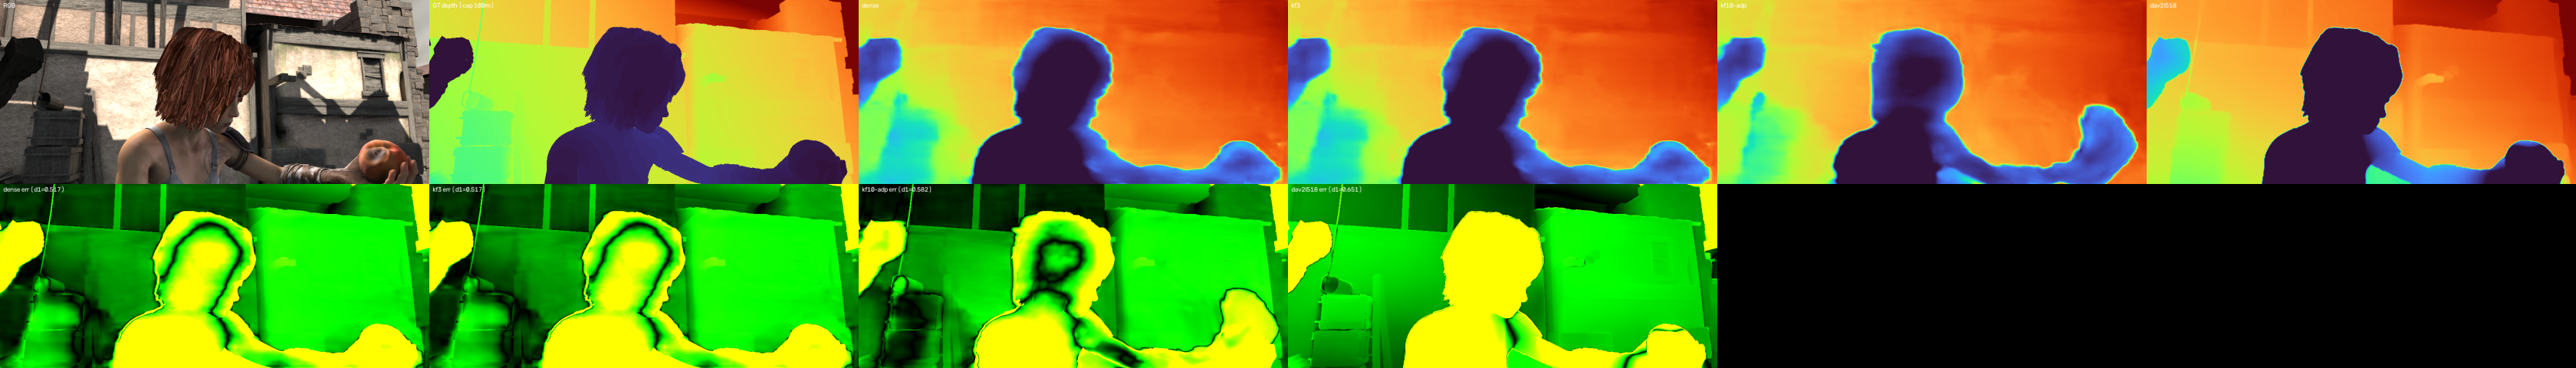
\includegraphics[width=\linewidth]{comparison_strip.png}\\[2pt]
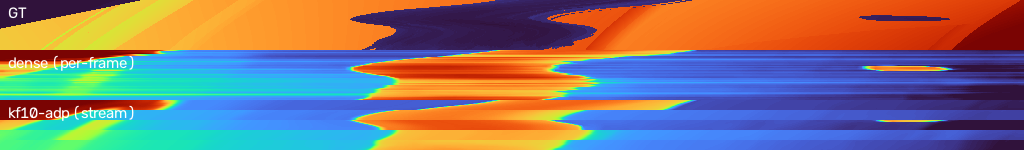
\includegraphics[width=\linewidth]{spacetime_slice.png}
\caption{\textbf{Qualitative comparison} (Sintel alley\_1). Top: RGB, ground
truth, and affine-aligned predictions of dense, kf3, kf10-adp, and the
teacher, with error maps ($\delta_1$ inset; green = accurate, red = $>25\%$
relative error). Bottom: \textbf{space-time slice} --- depth along one
scanline stacked over 50 frames. Per-frame inference (middle) flickers;
the stream (bottom) forms smooth bands.}
\label{fig:qual}
\end{figure}

\begin{figure}[t]
\centering
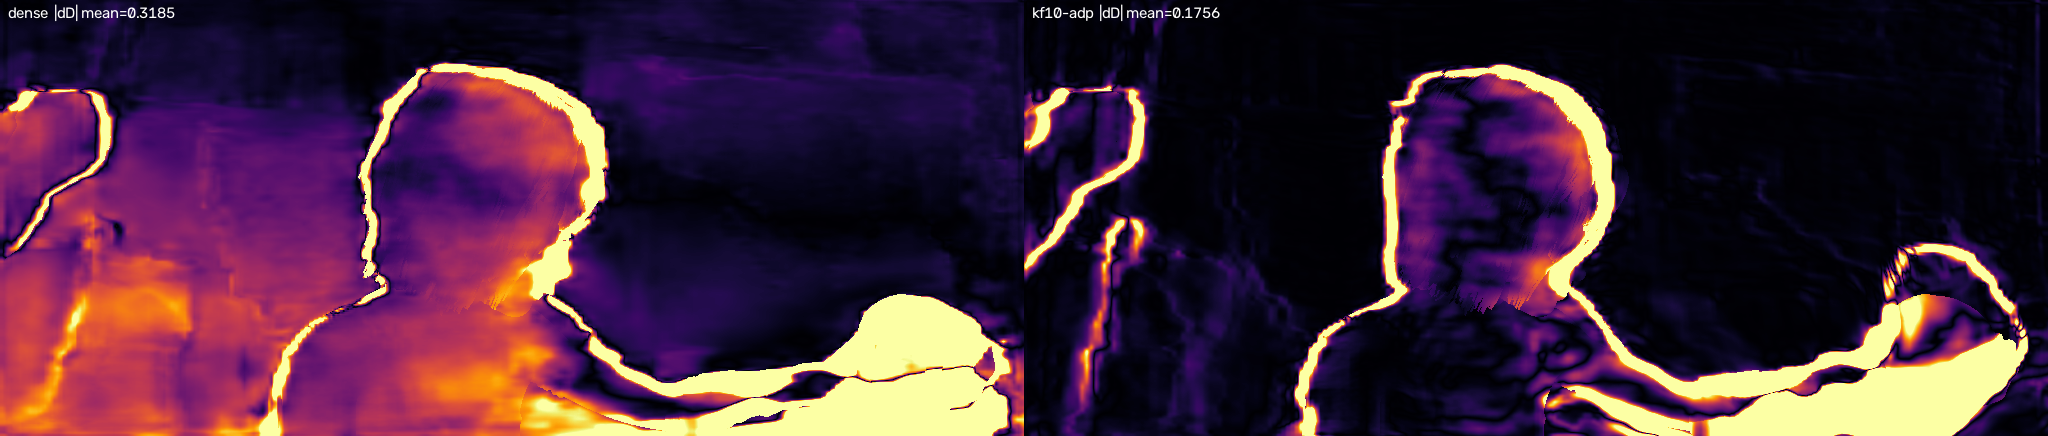
\includegraphics[width=\linewidth]{flicker_maps.png}
\caption{\textbf{Frame-to-frame flicker} $|D_t - \mathcal{W}(D_{t-1}, F^{gt})|$
(Sintel, GT-flow warp). Streaming reduces the mean flicker by 45\%
(0.3185 $\to$ 0.1756); residual error concentrates at motion boundaries ---
the expected failure mode of flow propagation.}
\label{fig:flicker}
\end{figure}

\begin{figure}[t]
\centering
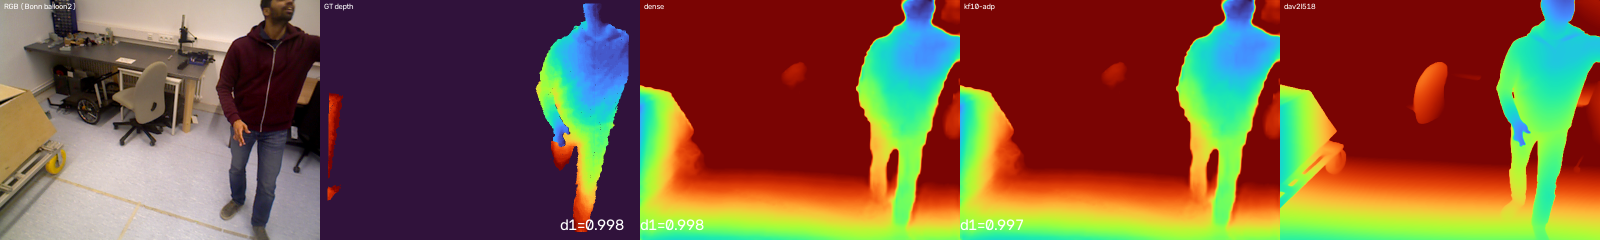
\includegraphics[width=\linewidth]{bonn_qual.png}
\caption{\textbf{Real data} (Bonn balloon2): RGB, Kinect ground truth, and
affine-aligned predictions. $\delta_1$ insets: 0.998 / 0.998 / 0.997.}
\label{fig:bonn}
\end{figure}

\begin{figure}[t]
\centering
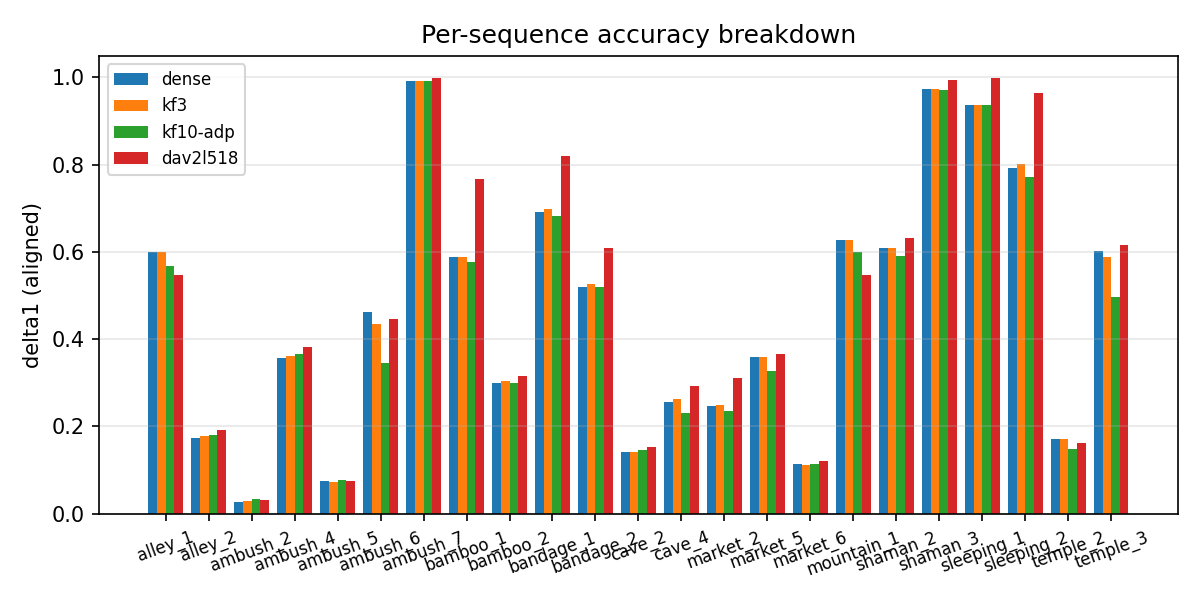
\includegraphics[width=0.8\linewidth]{perseq.png}
\caption{\textbf{Per-sequence accuracy} on Sintel (six-sequence protocol).
Sequence-level variance is dominated by scene difficulty (dense vegetation in
ambush sequences), not by the streaming mechanism.}
\label{fig:perseq}
\end{figure}

\subsection{Cadence sweep: choosing $K$}
\label{sec:ksweep}
Fig.~\ref{fig:ksweep} sweeps the cadence $K \in \{1,\dots,20\}$ over all 23
Sintel sequences. Latency falls steeply and then asymptotes
($12.4 \to 5.1$\,ms, a $2.4\times$ reduction bounded below by the flow term
of Eq.~\ref{eq:cost}), temporal error decreases monotonically --- longer
propagation chains are \emph{smoother} --- while accuracy degrades mildly
and non-monotonically (0.4614 at $K{=}1$ to 0.4297 at $K{=}20$, with a
recovery at $K{=}15$ that traces back to sequence-level variance rather
than to a resonance effect). The knee of the consistency--latency trade-off
sits at $K{\approx}10$, which we adopt as the default for adaptive
scheduling; $K{=}3$ is the accuracy-preserving alternative.

\begin{figure}[t]
\centering
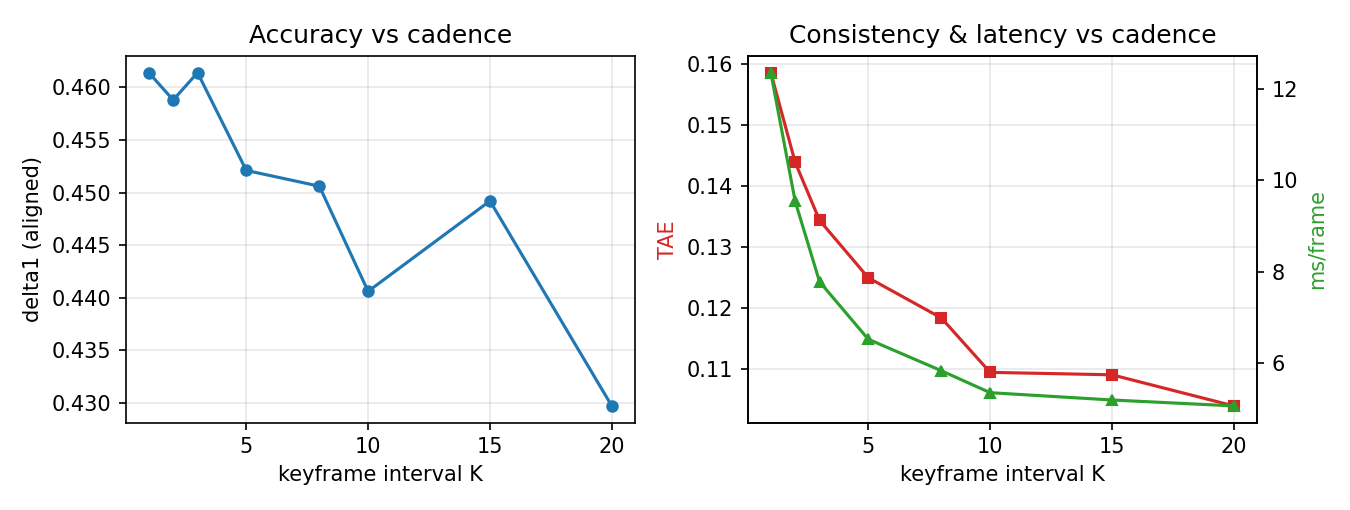
\includegraphics[width=\linewidth]{ksweep.png}
\caption{\textbf{Cadence sweep} (Sintel, 23 seq, TRT fp16). Left: accuracy
degrades mildly and non-monotonically with $K$. Right: temporal error
(TAE, GT flow) decreases monotonically while latency asymptotes to the
flow cost --- the knee sits at $K{\approx}10$.}
\label{fig:ksweep}
\end{figure}

\subsection{Comparing temporal stability with $\tau_5$}
\label{sec:tau5}
Table~\ref{tab:perseqfull} lists per-sequence accuracy for all
configurations; per-sequence variance (0.03 in ambush\_2 to 0.72 in
market\_6) is dominated by scene content, and the streaming configurations
track their dense counterpart within $\pm 0.02$ on 21 of 23 sequences.

\begin{table}[t]
\centering\footnotesize
\setlength{\tabcolsep}{3pt}
\caption{\textbf{Per-sequence $\delta_1$} on all 23 Sintel sequences
(GT-capped protocol, TRT fp16 backend).}
\label{tab:perseqfull}
\begin{tabular}{lcccc}
\toprule
Sequence & dense & kf3 & kf10 & kf10-adp\\
\midrule
alley\_1 & 0.5992 & 0.5985 & 0.5673 & 0.5673 \\
alley\_2 & 0.1741 & 0.1775 & 0.1796 & 0.1796 \\
ambush\_2 & 0.0263 & 0.0294 & 0.0327 & 0.0327 \\
ambush\_4 & 0.3564 & 0.3602 & 0.3033 & 0.3666 \\
ambush\_5 & 0.0760 & 0.0737 & 0.0766 & 0.0766 \\
ambush\_6 & 0.4611 & 0.4352 & 0.3449 & 0.3449 \\
ambush\_7 & 0.9920 & 0.9912 & 0.9908 & 0.9908 \\
bamboo\_1 & 0.5883 & 0.5877 & 0.5762 & 0.5762 \\
bamboo\_2 & 0.2989 & 0.3046 & 0.2989 & 0.2989 \\
bandage\_1 & 0.6911 & 0.6971 & 0.6823 & 0.6823 \\
bandage\_2 & 0.5193 & 0.5273 & 0.5196 & 0.5196 \\
cave\_2 & 0.1406 & 0.1408 & 0.1450 & 0.1450 \\
cave\_4 & 0.2565 & 0.2630 & 0.2310 & 0.2310 \\
market\_2 & 0.2462 & 0.2481 & 0.2350 & 0.2350 \\
market\_5 & 0.3585 & 0.3592 & 0.3264 & 0.3264 \\
market\_6 & 0.1140 & 0.1115 & 0.1128 & 0.1128 \\
mountain\_1 & 0.6276 & 0.6276 & 0.5998 & 0.5998 \\
shaman\_2 & 0.6095 & 0.6093 & 0.5897 & 0.5897 \\
shaman\_3 & 0.9737 & 0.9739 & 0.9700 & 0.9700 \\
sleeping\_1 & 0.9363 & 0.9376 & 0.9370 & 0.9370 \\
sleeping\_2 & 0.7923 & 0.8011 & 0.7706 & 0.7706 \\
temple\_2 & 0.1721 & 0.1701 & 0.1490 & 0.1490 \\
temple\_3 & 0.6030 & 0.5875 & 0.4958 & 0.4958 \\
\bottomrule
\end{tabular}
\end{table}

\begin{table}[t]
\centering\footnotesize
\caption{\textbf{Per-sequence $\delta_1$} on the 9 Bonn RGB-D sequences
(Kinect GT, TRT fp32 backend). crowd saturates the metric because its
consecutive Kinect frames are near-duplicates.}
\label{tab:bonnperseq}
\begin{tabular}{lccc}
\toprule
Sequence & dense & kf3 & kf10-adp\\
\midrule
balloon & 0.9999 & 1.0000 & 1.0000 \\
balloon2 & 0.9368 & 0.9378 & 0.9105 \\
balloon\_tracking & 0.9954 & 0.9958 & 0.9958 \\
balloon\_tracking2 & 0.9916 & 0.9918 & 0.9926 \\
crowd & 1.0000 & 1.0000 & 1.0000 \\
crowd2 & 0.9686 & 0.9623 & 0.9434 \\
crowd3 & 0.9999 & 0.9999 & 0.9999 \\
kidnapping\_box & 0.9964 & 0.9967 & 0.9960 \\
kidnapping\_box2 & 0.9911 & 0.9910 & 0.9914 \\
\bottomrule
\end{tabular}
\end{table}

TAE measures the magnitude of frame-to-frame drift; the propagation
literature additionally reports $\tau_5$
\cite{velodepth}, a per-pixel \emph{inlier rate}: depth from $t{-}1$ is
warped to $t$ (GT flow), scale--shift aligned per pair, and a pixel counts
as consistent when $|D_t - \widehat{D}_{t-1}| < 5\%$ of the depth. We
implement $\tau_5$ without the ego-motion term (our runtime consumes no
poses; the scale--shift alignment absorbs the dominant correction) and
report it for all Sintel configurations in Table~\ref{tab:tau5}. The
ordering matches TAE exactly, but the effect size is more readable:
streaming lifts the share of temporally consistent pixels from 55\%
(dense) to 73\% (kf3) and 83\% (kf10-adp) --- a $1.5\times$ improvement
that survives the switch to the rival metric family. Per-frame DAv2-L
scores 0.5516 under the same protocol.

\begin{table}[t]
\centering\small
\caption{\textbf{$\tau_5$ temporal consistency}. Top: Sintel (23 seq;
GT-flow warping). Bottom: Bonn (9 seq; estimated backward flow, identical
across configs). Per-pair scale--shift alignment, 5\% inlier threshold;
higher is better.}
\label{tab:tau5}
\begin{tabular}{lccc}
\toprule
Config & dense & kf3 & kf10-adp\\
\midrule
Sintel ($\tau_5{\uparrow}$) & 0.5516 & 0.7332 & \textbf{0.8303}\\
Bonn ($\tau_5{\uparrow}$) & 0.8737 & 0.8786 & \textbf{0.8854}\\
\bottomrule
\end{tabular}
\end{table}

\subsection{Platform and backend invariance}
Table~\ref{tab:platform} extends the evaluation across devices, from a
2019 \$99 developer board to a laptop GPU. The CPU runs the fp32 ONNX graph
(4 threads); INT8 dynamic quantization is counterproductive for this
convolutional model (82--144\,ms, a $12$--$20\times$ slowdown, because
dynamic quantization falls back to slow reference kernels), though it
shrinks the artifact to 6\,MB. Three claims matter for deployment:
(i)~\emph{accuracy is backend-invariant} --- over all configurations the
fp32-CPU and fp16-GPU predictions agree to $\delta_1 \leq 10^{-4}$;
(ii)~\emph{amortization flips the CPU calculus} --- with the student's cost
amortized over ten frames, the CPU stream is not merely real-time
(249\,FPS end-to-end at $640{\times}480$) but \emph{faster} than the GPU
stream, because flow and warping dominate the per-frame budget once
inference is amortized away; and (iii)~\emph{2019 hardware streams in real
time} --- on a Jetson Nano 4GB (Maxwell GPU, 4\,GB shared memory), per-frame
inference reaches only 21\,FPS at $640{\times}480$, below the real-time
line, while DepthStream kf10 runs at 90\,FPS ($4.2\times$; the full cadence
sweep 21/48/90/90\,FPS traces the amortization curve on
Fig.~\ref{fig:pareto}) --- the same
runtime whose closest learned-propagation competitor~\cite{velodepth}
targets an RTX~3090. Cross-device agreement of the streamed fields
(Nano TRT fp32 vs.\ desktop ORT fp32, 30 frames) is Pearson $r{=}0.956$;
the residual gap reflects platform-specific engine kernels and flow-level
numerics, both invisible to the affine-invariant protocol of
Tables~\ref{tab:main} and~\ref{tab:ablation}.

\begin{table}[t]
\centering\small
\caption{\textbf{Platforms} (student backend; E2E on a $640{\times}480$
synthetic clip, kf10, MAXN power mode). Nano cadence sweep
(per-frame/kf3/kf10/kf10-adp): 47.2/20.9/11.2/11.2\,ms
= 21.2/47.9/89.6/89.6\,FPS (see also Fig.~\ref{fig:pareto}).
Backend invariance: $|\Delta\delta_1| \leq 10^{-4}$ between GPU-fp16 and
CPU-fp32 on the Sintel protocol.}
\label{tab:platform}
\begin{tabular}{llccc}
\toprule
Platform & Backend & Prec. & model & E2E kf10\\
\midrule
RTX 3060 Laptop 6GB & TensorRT 11.3 & fp16 & 1.20\,ms & $\sim$150 FPS\\
Ryzen 7 5800H (CPU) & ORT 1.26 & fp32 & 6.95\,ms & 249 FPS\\
Jetson Nano 4GB (2019) & TensorRT 8.2 & fp32 & 29.9\,ms & 90 FPS\\
\bottomrule
\end{tabular}
\end{table}

\begin{table}[t]
\centering\small
\caption{\textbf{Per-component budget} (ms; $640{\times}480$). model = one
student call as executed by the runtime (preprocess + host--device transfer
+ engine); flow = one DIS field at 256\,px incl.\ upsampling; warp =
full-resolution remap. At $224^2$ the Python-side preprocessing dominates
the model call on every platform.}
\label{tab:components}
\begin{tabular}{lccc}
\toprule
Platform & model & flow & warp\\
\midrule
RTX 3060 Laptop (TRT fp16) & 12.4 & 2.2 & 0.8\\
Ryzen 7 5800H (ORT fp32) & 12.1 & 2.2 & 0.7\\
Jetson Nano (TRT fp32) & 46.6 & 7.3 & 1.0\\
\bottomrule
\end{tabular}
\end{table}

\subsection{Analysis: when does selective refinement pay off?}
\label{sec:cascade}
A natural competitor to amortization is \emph{selection}: run the large
teacher only where the small model is expected to err. We built this
speculative-cascade runtime (flip-consistency and edge cues select the top
$p\%$ of $16{\times}16$ blocks; the teacher runs on the selected crops;
crops are affine-aligned on their rings and feather-blended). On Sintel, the
student already agrees with the teacher on 93.6\% of pixels ($\delta_1$
against the teacher as reference), and every cascade budget we tested
(10/20/40\%) \emph{lost} accuracy against the pure student while costing
$70\times$ more latency --- crop-level ViT-L inference cannot amortize below
a single full-image forward pass on this hardware. The negative result is
informative: distilled students leave no disagreement space for a teacher to
arbitrate, which is precisely why propagation-based systems over
\emph{non-distilled} foundation models~\cite{velodepth} require learned
corrections. Selection, not amortization, is the right tool for
foundation-model students; amortization is the right tool for distilled ones.

\subsection{Negative result: homography-based geometric propagation}
We additionally implemented a geometric variant: RANSAC homography on sparse
flow correspondences, homography warping on static-inlier regions, flow
elsewhere. It improves the single rotation-dominated sequence (temple\_2,
$+13\%$ relative $\delta_1$) but loses overall (0.2776 vs.\ 0.2827 mean on a
four-sequence pilot): Sintel's camera motion is dominated by forward
translation with strong parallax, which a single global homography cannot
represent, while dense backward flow covers translation and rotation
uniformly. Dense learned-free flow is a strong propagator precisely because
it makes no motion-model assumption.

%--------------------------------------------------------------------------
\section{Discussion}
\label{sec:discussion}

\subsection{DepthStream vs.\ learned propagation}
Table~\ref{tab:velodepth} summarizes the contrast with the closest system.
The two approaches are complementary rather than competing: VeloDepth
demonstrates that learned corrections squeeze extra consistency out of a
\emph{non-distilled} foundation base, while DepthStream shows that for
students distilled from the judge model, the same skeleton --- keyframe,
warp, re-anchor --- delivers a large share of the benefit with no training
pipeline, an order of magnitude lower latency, and $7\times$ smaller
hardware. The practical decision rule that emerges from our analysis
(Sec.~\ref{sec:cascade}) is: \emph{if your tiny model is distilled from your
quality reference, propagate --- do not correct; and re-anchor --- do not
smooth.}

\begin{table}[t]
\centering\small
\caption{\textbf{DepthStream vs.\ learned propagation} (VeloDepth numbers
from their paper; both on 0.3--0.5\,MP inputs).}
\label{tab:velodepth}
\begin{tabular}{lcc}
\toprule
 & VeloDepth & DepthStream (ours)\\
\midrule
propagation module & 55\,M, trained & none\\
training cost & 8$\times$4090, 6 days & ---\\
base model & 409\,M (UniDepthV2) & 6\,M distilled\\
keyframe trigger & learned gating & residual (free)\\
hardware & RTX 3090 & RTX 3060 Laptop 6GB\\
throughput & 26.2 FPS & 142--176 FPS\\
\bottomrule
\end{tabular}
\end{table}

\subsection{When does amortization stop paying?}
Three boundaries emerged from our experiments. \emph{Occlusion density}:
propagation error concentrates at disocclusions (Fig.~\ref{fig:flicker});
adaptive scheduling hides the symptom at scene level but a per-pixel mask
with fallback inference is the natural next step. \emph{Extreme intervals}:
beyond $K{\approx}15$ the accumulation curve (Fig.~\ref{fig:accum}) falls
below the dense baseline, so the cadence should stay within the range where
decay is flatter than the model's own frame-to-frame variance ---
empirically $K{\leq}10$ here. \emph{Model mismatch}: if the runtime's
student is \emph{not} distilled from the referee model, a disagreement
space re-opens and selective correction (Sec.~\ref{sec:cascade}) or learned
propagation~\cite{velodepth} becomes rational again.

%--------------------------------------------------------------------------
\section{Limitations}
\label{sec:limits}
(i) Flow propagation fails at disocclusions and large rotations; the adaptive
scheduler masks the symptom (early re-anchoring) but does not model
occlusion explicitly. (ii) Our evaluation covers one synthetic and nine real
sequences; extending Bonn to all published sequences and adding TUM would
strengthen the real-data claim. (iii) Power consumption is not yet reported
for the platform table, and GPU-side evaluation uses one consumer laptop GPU;
Orin-class Jetson results are expected to transfer directly (same TensorRT
pipeline, official DepthART scripts exist). (iv) The student consumes no
camera intrinsics here; the metric variant of DepthART would require
propagating $K$ jointly with the field. (v) VeloDepth~\cite{velodepth}
reports a temporal-consistency metric ($\tau^{\mathrm{SSI}}_5$) that we have
not yet reproduced, so our comparison to it is architectural and
latency-based rather than metric-exact.

%--------------------------------------------------------------------------
\section{Conclusion}
DepthStream turns a distilled 6\,M-parameter depth model into a temporally
stable, full-resolution video depth stream --- without training anything.
The runtime amortizes the student across frames with backward-flow
propagation, re-anchors fresh predictions with a closed-form affine fit, and
schedules keyframes with a photometric failure detector. On synthetic and
real benchmarks it matches per-frame accuracy at moderate intervals, beats
per-frame temporal stability by $1.75\times$ relative to a teacher $6.7\times$
slower, reaches 249\,FPS on a CPU, and stays accuracy-invariant across
backends. Beyond the system, our analysis gives practitioners a simple
decision rule: if your tiny model is distilled from your judge model,
propagate --- do not correct; and do not smooth --- re-anchor.

%--------------------------------------------------------------------------
\section*{Reproducibility and licensing}
All tables are produced by single commands
(\texttt{eval\_sintel\_v2.py}, \texttt{eval\_bonn.py}, \texttt{bench\_cpu.py};
figures by \texttt{plots.py}, \texttt{qual\_figs.py}, and
\texttt{draw\_framework.py}). The student checkpoint and teacher weights are
public; the student and parts of its supervision inherit CC BY-NC 4.0 terms
from DepthART and Depth Anything V2, which restricts commercial use of the
released weights (the runtime itself has no such restriction). Sintel and
Bonn are used under their respective research licenses.

\begin{thebibliography}{25}\small
% TODO: verify all entries (venue/year/ids) before submission.
\bibitem{depthart} F.~Xue et al.
``DepthART: Scaling Foundation Monocular Depth to Tiny Models,''
\emph{ACM Multimedia}, 2026. arXiv:2607.17099.
\bibitem{dav2} L.~Yang et al.
``Depth Anything V2,'' \emph{NeurIPS}, 2024. arXiv:2406.09414.
\bibitem{velodepth} L.~Piccinelli et al. ``Video Depth Propagation
(VeloDepth),'' \emph{3DV}, 2026. arXiv:2512.10725.
\bibitem{nvds} W.~Wang et al. ``Neural Video Depth Stabilizer,''
\emph{ICCV}, 2023.
\bibitem{depthcrafter} W.~Cao et al. ``DepthCrafter: Generating Consistent
Long Depth Sequences for Open-world Videos,'' \emph{CVPR}, 2025.
\bibitem{chronodepth} J.~Shao et al. ``Learning Temporally Consistent Video
Depth from Video Diffusion Models'' (ChronoDepth), \emph{CVPR}, 2025.
\bibitem{vda} S.~Chen et al. ``Video Depth Anything: Consistent Depth
Estimation for Super-Long Videos,'' \emph{CVPR}, 2025. arXiv:2501.12375.
\bibitem{cvd} J.~Kopf et al. ``Consistent Video Depth Estimation,''
\emph{ACM TOG (SIGGRAPH)}, 2021.
\bibitem{teccvideodepth} S.~Li, Y.~Luo, Y.~Mao et al. ``Enforcing Temporal
Consistency in Video Depth Estimation'' (TCMonoDepth), \emph{ICCV Workshops},
2021.
\bibitem{midas} R.~Ranftl et al. ``Towards Robust Monocular Depth Estimation:
Mixing Datasets for Zero-shot Cross-dataset Transfer,'' \emph{IEEE TPAMI},
2022.
\bibitem{da1} L.~Yang et al. ``Depth Anything: Unleashing the Power of
Large-Scale Unlabeled Data,'' \emph{CVPR}, 2024. arXiv:2401.10891.
\bibitem{zoedepth} S.~F.~Bhat et al. ``ZoeDepth: Zero-shot Transfer by
Combining Relative and Metric Depth,'' \emph{ICRA}, 2023.
\bibitem{marigold} B.~Ke et al. ``Repurposing Diffusion-based Image
Generators for Monocular Depth Estimation,'' \emph{CVPR}, 2024.
\bibitem{depthfm} M.~Gui et al. ``DepthFM: Fast Monocular Depth Estimation
with Flow Matching,'' \emph{ACM Multimedia}, 2024.
\bibitem{rtmonodepth} M.~Pietruszka et al. ``Real-Time Monocular Depth
Estimation on Embedded Systems,'' \emph{arXiv:2308.10569}, 2023.
\bibitem{dff} X.~Zhu et al. ``Deep Feature Flow for Video Recognition,''
\emph{CVPR}, 2017.
\bibitem{xmem} C.~Cheng and M.~Schiele. ``XMem: Long-Term Video Object
Segmentation with an Atkinson-Shiffrin Memory Model,'' \emph{ECCV}, 2022.
\bibitem{specdec} Y.~Leviathan et al. ``Fast Inference from Transformers via
Speculative Decoding,'' \emph{ICML}, 2023.
\bibitem{practicalcvd} P.~Li, Y.~Ding, L.~Li, J.~Guan, and Z.~Li. ``Towards
Practical Consistent Video Depth Estimation,'' \emph{ACM ICMR}, 2023.
\bibitem{metric3d} W.~Yin et al. ``Metric3D v2: Geometric Foundation Model,''
\emph{IEEE TPAMI}, 2024.
\bibitem{unidepth} L.~Piccinelli et al. ``UniDepth: Universal Monocular
Metric Depth Estimation,'' \emph{CVPR}, 2024.
\bibitem{fastdepth} D.~Wofk et al. ``FastDepth: Efficient Monocular Depth
Estimation for Embedded Devices,'' \emph{ICRA}, 2019.
\bibitem{patchfusion} Z.~Li et al. ``PatchFusion: An End-to-End Tile-Based
Framework for High-Resolution Monocular Metric Depth Estimation,''
\emph{CVPR}, 2024.
\bibitem{disflow} T.~Kroeger et al. ``Fast Optical Flow using Dense Inverse
Search,'' \emph{ECCV}, 2016.
\bibitem{farneback} G.~Farneb\"ack. ``Two-Frame Motion Estimation Based on
Polynomial Expansion,'' \emph{SCIA}, 2003.
\bibitem{sintel} D.~J.~Butler et al. ``A Naturalistic Open Source Movie for
Flow Evaluation,'' \emph{ECCV}, 2012.
\bibitem{bonn} E.~Palazzolo et al. ``ReFusion: 3D Reconstruction in Dynamic
Environments using a Time-of-Flight Sensor'' (Bonn RGB-D Dynamic), \emph{IROS},
2019.
\bibitem{dpt} R.~Ranftl et al. ``Vision Transformers for Dense Prediction''
(DPT), \emph{ICCV}, 2021.
\bibitem{mobilenetv4} D.~Qin et al. ``MobileNetV4 -- Universal Models for the
Mobile Ecosystem,'' \emph{arXiv:2404.10518}, 2024.
\bibitem{tensorrt} NVIDIA. ``TensorRT,'' \url{https://developer.nvidia.com/tensorrt}.
\end{thebibliography}

\end{document}
